\documentclass[12pt,tikz]{standalone}

\usepackage{graphicx}
\usetikzlibrary{positioning}
\begin{document}

\newcommand{\state}[2]{%
  $s = $ \texttt{#1}\\
  $p = $ \texttt{#2}
}

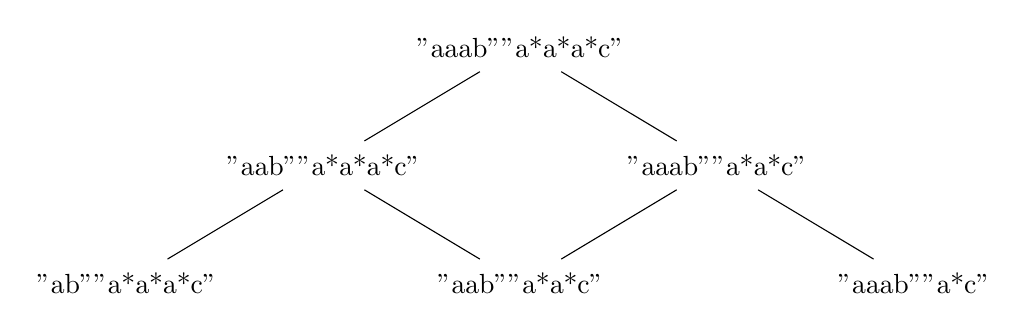
\begin{tikzpicture}[align=center, draw, black, shorten >=3pt, shorten <=3pt, node distance = 1.5cm]
  \node at (5, 0) (root) {\state{"aaab"}{"a*a*a*c"}};
  \node at (2.5, -1.5) (L) {\state{"aab"}{"a*a*a*c"}};
  \node at (7.5, -1.5) (R) {\state{"aaab"}{"a*a*c"}};
  \node at (0, -3) (LL) {\state{"ab"}{"a*a*a*c"}};
  \node at (10, -3) (RR) {\state{"aaab"}{"a*c"}};
  \node at (5, -3) (mid) {\state{"aab"}{"a*a*c"}};

  \draw (root) -- (L);
  \draw (root) -- (R);
  \draw (L) -- (LL);
  \draw (R) -- (RR);
  \draw (L) -- (mid);
  \draw (R) -- (mid);
\end{tikzpicture}
\end{document}

